%Edit 0033 ZZZ to report number nnnn 
%Edit 3.4 YYMILE to milestone number m.m.m
%Edit Development plan YYTITLE to report title - Words Start with Caps
\documentclass[11pt,twoside,a4paper]{article}
%%======================================================================
%% PACKAGES:
%%
%\usepackage{times}               % Times+Helvetica+Courier fonts
\usepackage{helvet}              % helvetica + cmr
\usepackage{fancyhdr}       % package for headers/footers
\usepackage{amsmath}
\usepackage{amssymb}
\usepackage{graphicx}            % Graphics.
%\usepackage{a4}                  % page layout to fit A4
%\usepackage{lastpage}            % get page no of last page
%\usepackage{ifthen}              % logical branching
\usepackage{hyperref}            %insert hyper-links
\usepackage{latexsym}
% uncomment the following to override auto page total
%\pptotal{20}
%%======================================================================

% ensure sans-serif font used throughout
\renewcommand{\familydefault}{\sfdefault}

\newcommand{\culhamissueno}{1.00}%<==edit
\newcommand{\culhamshorttitle}{CD/EXCALIBUR-FMS/0033}%<==edit
\newcommand{\Sec}[1]{Section~\ref{sec:#1}}
\newcommand{\Fig}[1]{Figure~\ref{fig:#1}}
\newcommand{\Tab}[1]{Table~\ref{tab:#1}}
\newcommand{\Eq}[1]{Equation~(\ref{eq:#1})}
\newcommand{\Eqs}[2]{Equations(\ref{eq:#1}) and~(\ref{eq:#2})}
\newcommand{\Figs}[2]{Figures~\ref{fig:#1}--~\ref{fig:#2}}
%Bold lc for script names, tt for computer code and file-names
%\F{NEPTUNE} always in caps
\newcommand{\F}[1]{\textsc{#1}}
\newcommand{\B}[1]{\textbf{#1}}
\newcommand{\T}[1]{\texttt #1}
\newcommand{\V}[1]{\mathbf{#1}}
\newcommand{\I}[1]{\textit{#1}}
\newcommand{\nep}{\textsc{NEPTUNE}}
\newcommand{\exc}{\textsc{E}x\textsc{CALIBUR}}
\newcommand{\Papp}{Proxyapp}
\newcommand{\papp}{proxyapp}



%%======================================================================

%% REPORT COVER PAGE Information

\newcommand{\culhamtitle}{\LARGE Development plan  \\[1.0\baselineskip] D3.4 }%<==edit

%%QA BOX information -- change following as needed
\newcommand{\culhamboardname}{Martin O'Brien}%<==edit
\newcommand{\culhamcontactname}{Rob Akers}%<==edit
\newcommand{\culhamauthor}{Wayne Arter}%<==edit
\newcommand{\culhamauthora}{Ed Threlfall}%<==edit
\newcommand{\culhamauthorb}{Joseph Parker}%<==edit
\newcommand{\culhamauthorc}{Will Saunders}%<==edit
%\newcommand{\culhamcontacttel}{Telephone: 01235 466498}
%\newcommand{\culhamcontactemail}{Email: rob.akers@ukaea.uk}

\newcommand{\culhamdate}{16 March 2021}%<=edit
\newcommand{\culhamdatea}{16 March 2021}%<=edit
\newcommand{\culhamdateb}{16 March 2021}%<=edit

% reproduce Rob's page size

\setlength{\textheight}{220.0mm}
\setlength{\textwidth}{165.0mm}
\setlength{\topmargin}{0.0mm}
\setlength{\oddsidemargin}{0.0mm}
\setlength{\evensidemargin}{\oddsidemargin}
\setlength{\parindent}{0mm}
\addtolength{\parskip}{0.5\baselineskip}
\setlength{\topsep}{0pt}
\setlength{\itemsep}{0pt}

%%======================================================================
\begin{document}

%Titlepage comes out wrong size, but should look right apart from
% picture which cannot be wider than c.150mm.
% To produce conforming report rp1pub.pdf
% remove title page by commenting out lines ending in %<==omit, then
% sed -e '/<==omit$/s/^/%/' < rp1.tex > rp1omit.tex
% pdflatex rp1omit;bibtex rp1omit; pdflatex rp1omit
% pdfunite cover.pdf rp1omit.pdf rp1pub.pdf 
\begin{titlepage}%<==omit
\vspace*{-30mm}%<==omit

\includegraphics[width=2.5cm]{../corpics/cofaplus} \\[2.0\baselineskip]%<==omit
{\LARGE {\textbf{\textsf{ExCALIBUR}}}}\\[2.0\baselineskip]%<==omit
{\LARGE \culhamtitle } \\[2.0\baselineskip]%<==omit
{\textbf{\textsf{Abstract}}}\\%<==omit
The report describes work for \exc \ project \nep \ %<==omit
at the point of Deliverable D3.4. %<==omit
This report provides a discussion for the \nep\ project
of both very high-level and very low-level options for the basic module structure,
together with input/output and fine-scale data structures.
It complements the description provided by the previous milestone
reports~\cite{y1re331,y2re332,y2re333}.
This report completes D3.3 to produce a background against which final decisions may be taken
regarding decomposition of \nep\ software into modules,
and the grouping of modules into packages. It recommends use of the
Unified Modeling Language~(UML~2) to describe software structure.
%<==omit
%<==omit
\vfill%<==omit
\centerline{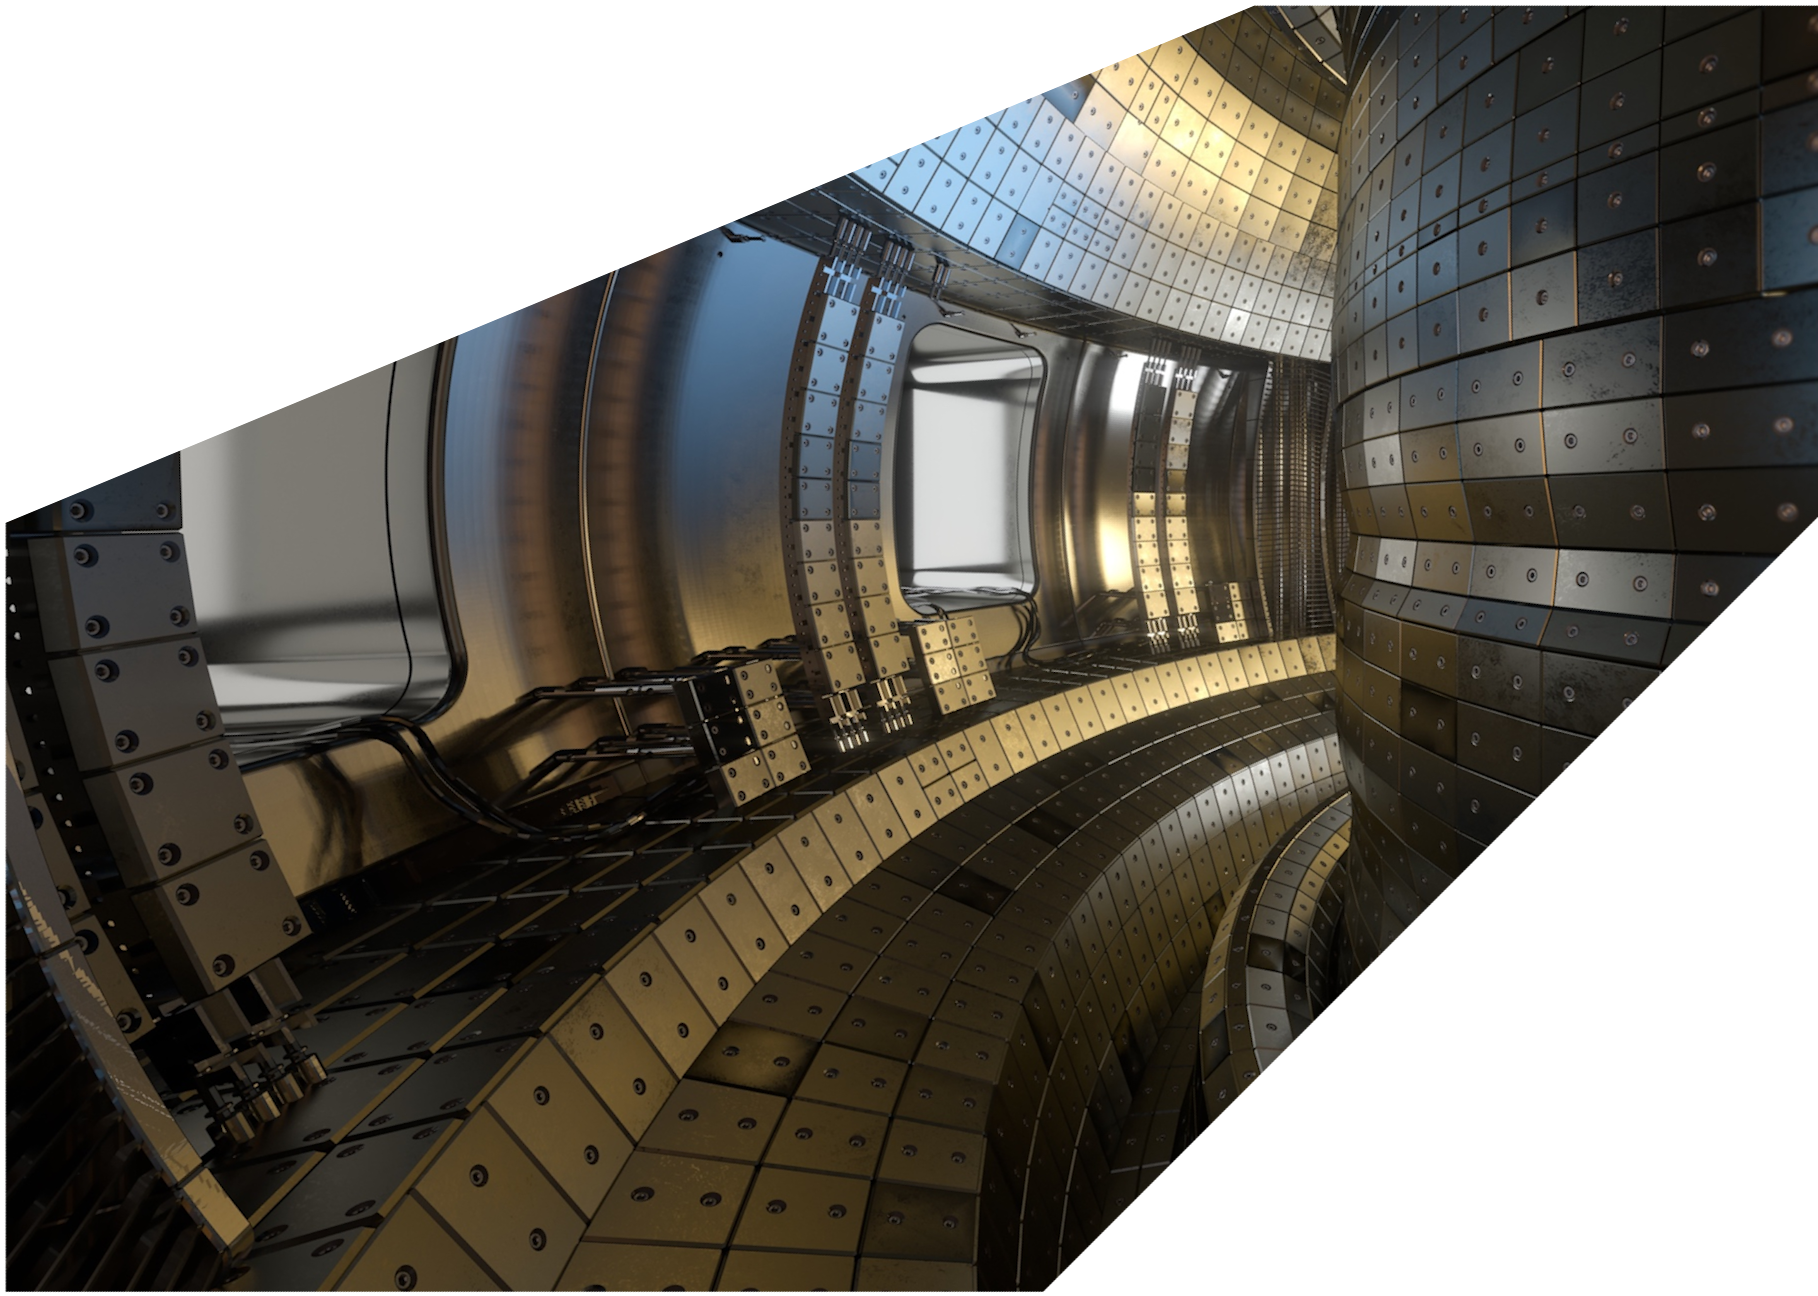
\includegraphics[width=0.9\textwidth]{../corpics/tokintcrop}}%<==omit
\end{titlepage}%<==omit

\hspace{-30mm}\begin{table}[h]
\sffamily
\begin{center}
\textbf{\textsf{UKAEA REFERENCE AND APPROVAL SHEET}}
\begin{tabular}{||p{5.7cm}|p{4.7cm}|p{5.0cm}||}
\hline
\hline
& Client Reference: &  \\
\hline
& UKAEA Reference: & \culhamshorttitle \\
& & \\
\hline
& Issue: & \culhamissueno \\
\hline
& Date: & \culhamdateb \\
\hline
\multicolumn{3}{||l||}{} \\
\multicolumn{3}{||l||}{Project Name: ExCALIBUR Fusion Modelling System} \\
\multicolumn{3}{||l||}{} \\
\hline
\end{tabular}
\begin{tabular}{||p{3.3cm}|p{4.6cm}|p{3.5cm}|p{3.6cm}||}
\hline
& Name and Department & Signature & Date \\
\hline
Prepared By: & \culhamauthor & N/A & \culhamdate \\
& \culhamauthora & N/A & \culhamdate \\
& \culhamauthorb  & N/A & \culhamdate \\
& \culhamauthorc  & N/A & \culhamdatea \\
& & & \\
& BD & & \\
\hline
Reviewed By: & \culhamcontactname & 
\includegraphics[width=3.0cm]{../corpics/blanksign}& \culhamdatea \\
& & & \\
& Advanced Computing Dept. Manager & & \\
\hline
Approved By: & \culhamboardname  & 
\includegraphics[width=3.0cm]{../corpics/blanksign} & \culhamdateb \\
& & & \\
& MSSC & &\\
\hline
\hline
\end{tabular}
\end{center}
\end{table}


\clearpage
\section{Introduction}\label{sec:intro}
Drawing on the lessons learnt from earlier \nep\ work, especially ref~\cite{y2re312}, not only will the
software will be opensource, but in the interests of encouraging as wide a possible range of developers,
\nep\ will be treated as a community project with maximal transparency regarded decision-making, resource allocation etc.
Successful examples of such projects set out principles that community members are expected to adhere to,
and guidelines for them to follow. This amounts to significantly more detail both concerning the
management of the development and the production of the software, than appears in the \nep\ Science Plan
and Charter~\cite{sciplan,charter} and the subsequent initial reports~\cite{y1re311,y1re331}. 

The present report looks in detail at a number of sources recommending what documents are required
for the successful conduct of a software development project. Following from the report~\cite{y1re311},
the first of these is the book chapter by Spencer Smith~\cite{Sm17Rati},
as specifically directed to \emph{scientific} software.
The conclusion of the report~\cite[\S\,3]{y2re312} draws attention to Sommerville~\cite{sommerville10}
who has relevant material dispersed throughout the book and Hewitt~\cite{hewittexc}, although these
are aimed at a wider, more commercially-oriented range of developments. Focussing on science,
specifically space applications
there is the European Space Agency~(ESA) standards document~\cite{ecss40exc} which in
a ``lite" form has proved successful in two 
UKAEA developments this century, viz.\ \F{FISPACT}~\cite{Su17FISP} and \F{SMARDDA}~\cite{Wa15}.

None of these sources is entirely suitable for \nep. 
The proposed ``faking" of documents by Smith seems unsatisfactory. Hurried writing  is suggested
by the inconsistency
between his statements that no-one likes documenting software and his recommendations that more
documents be produced, a suggestion supported by the fact that the proposed division
of material between various documents seems unsatisfactory in some places, eg.\ where the
functional and nonfunctional requirements are combined together in one section of a document
entitled the ``Software Requirements Specification". As a text-book, Sommerville offers a multitude
of possibilities, but few are relevant to open-source scientific software; therefore Hewitt scores
by being more focussed and by an emphasis on awareness of the surrounding business environment.
The ESA approach does not meet \nep\ needs in that it assumes a single expert customer
for the project, and anyway
the full standard, intended for flight-critical software, is arguably too onerous, where the
``lite" version is more appropriate for a contractor with a single worker.

In addition to the points in the preceding paragraph, none of the sources fully addresses the issue
that scientist developers do not like producing documentation. Ideally, material should be written up
only once to be presented to developers and users of whatever level of competence as appropriate. This
is probably best addressed by producing documentation as web pages, as indeed indicated by both Spencer Smith
and Hewitt.
%Moreover to minimise documentation writing for \nep, the arrangement of these web pages
%into a public website for the code  ought to be considered at the outset. To this end, the structure
%of the plasmapy website~\cite{plasmapywebsite} has been studied, particularly the documentation.

The main \Sec{taskwork} provides a concordance of the documents from the
texts~\cite{hewitt, Sm17Rati, sommerville10} in \Sec{concord}, then gives more details
as to what information should be provided in each in \Sec{detailedinfo}. It is followed by
discussion of how best to format the documentation as a website in \Sec{toweb}.




\clearpage
\section{Task Work}\label{sec:taskwork}
\subsection{General Considerations}\label{sec:considers}
It is important that individual
units of code are manageable and the overall structure is comprehensible,
so that developers and users can navigate the codebase and determine where new work is to be located.
This simple consideration implies that \nep\ software
should be divided into units that it will be convenient to refer
to as modules,
sections of code containing everything necessary to perform one (and only one)
aspect of the desired functionality.

The suggested content of a module
describing a single class in the UML sense (see \Sec{lowlevel}, \Tab{umltrans})
implies a minimum of $13$~methods described by separate Fortran subroutines,
with examples extending up to $50$, although the latter is there regarded as an excessively large
number of methods..
Many small software libraries also fall into this size range.
Supposing that each subroutine is of a length to fit within one computer window, ie.\
up to about~$60$~lines, the desirable maximum length of a well-designed module file is
$30\times60 = 1\,800$~lines which is a manageable size of file given 
editing software that remembers on restart, the last line accessed (so that it possible
to return immediately to a particular subroutine).
The magnitude of the D3.3 exercise follows from
the fact that comparable software packages probably of somewhat lesser complexity
than \nep\ written in high level languages such as C++ range in size up to~$1\,000\,000$ lines.
Clearly $400$~separate modules is too unwieldy, and there is a need to organise
further into packages which might contain in turn $10$-$50$ modules. 
As a way of providing further indication to developers,
it is helpful to talk of packages as being arranged into layers, as discussed
in ref~\cite[\S\S\,2.4,3.2]{y2re333}, see \Fig{hierarchygroup}.
Then, as prefigured in ref~\cite[Annex~A]{y2re333}, it is possible to encapsulate
the necessary complexity in one, albeit large diagram.
\begin{figure}
\centerline{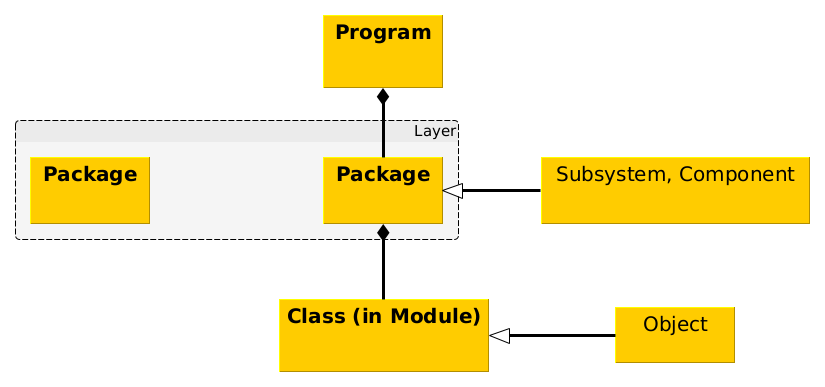
\includegraphics[width=0.7\textwidth]{../png/hierarchygroup}}
\caption{
Sketch of relationship between units of large code.
\label{fig:hierarchygroup}}
\end{figure}

\subsection{Considerations for Scientific Software}\label{sec:scistruct}
\subsubsection{Structural Considerations}\label{sec:structure}
In both refs~\cite{y1re331,y2re332}, a figure from Dubey~et~al~\cite{Du16Idea} is reproduced
that illustrates how scientific software may be developed by beginning with an ``infrastructure"
capability into which initially exploratory scientific software is integrated as its worth
is established. Unfortunately for \nep, it is not clear initially what  aspects  of the infrastructure
will be durable and stable, although once the software is more mature, Dubey~et~al's methodology
appears attractive.

The literature referenced in ref~\cite{y2re333} and indeed the local practice of the \F{SMARDDA} development
indicates that scientific software should be produced by aggregation, but are less
helpful as to what is to be aggregated, i.e.\ the modular decomposition as to what should
constitute a single module etc. Surprisingly little detailed discussion was found in the literature
after the early book by Booch~\cite{booch}, as to how to create classes in
the scientific and engineering context, with the exception of Douglass~\cite[\S\,5]{douglass}.
The ideal would be a way to create classes that enabled rapid development  of code
that executed efficiently but was easily re-used.
%where flexibility is also an important consideration,
Douglass~\cite[\S\,5]{douglass} does not specifically address these last points, but they
could guide choice of objects in his approach which is reproduced as Appendix~\Sec{objdisc}.

The \nep\ development will proceed as a series of \papp s. Thus there is a chance
to refine and redefine an initial modular decomposition with each successive \papp,
recording the results as a UML structure diagram. When generating the corresponding
sequence diagram (i.e.\ procedural description), the \papp-based units should be preserved to
facilitate the use of the simpler ones as surrogates for the later more complex \papp s.

To help understand the  aggregation of the software, it should be layered in the obvious manner,
with the higher layers corresponding to greater numbers of aggregated objects. It is also expected
to be useful to classify the modules.
The modules should be arranged into a relatively small number of packages according to, for example,
whether they treat
geometry generation, matrix coefficient calculation, the main matrix solution, or visualisation.
%\clearpage
\subsubsection{Interactions between Modules}\label{sec:modulint}
Concerning logical interconnections between modules, the 
use of  a directed, acyclic graph~(DAG) structure might be thought mandatory,
particularly to  process the input
data in order to specify coherently the construction of the elements of the solution matrix.
However, as prefigured in ref~\cite{y2re333} for the gyrokinetics code \F{GS2}, the tightly coupled nature of the central edge
physics problem  means that input is more about gathering \emph{all} the data, for only at that point
can fields be computed and only after that may matrix coefficients be computed.

\subsection{Design of a Module}\label{sec:lowlevel}
\subsubsection{Notation}

It should be noted that when discussing software in text documents,
the following conventions in \LaTeX\  are used
\begin{itemize}
\item \F{Small capitals} denote a package name
\item \I{Italics} denote a program name
\item \T{Fixed width font} denotes any code name or fragment which is not otherwise obviously source code
\item \B{Bold} denotes a shell script name
\end{itemize}
However special fonts are not employed if the class is identified by a
suitable suffix, thus ``\_m" for a module containing executable code defining methods,
``\_h" or ``.h" for class attributes (equivalently derived type or namespace code), ``.cpp" for name of file containing 
C++ source, ``.exe" for an executable, etc.
%Note that Object Fortran has led the way in that 
%requires only one copy of a class's attributes to be compiled, whereas only the very latest versions of C++
%avoid recompilation of namespaces when a .cpp file is changed.
UML nomenclature
is preferred herein, for which \Tab{umltrans} provides a limited 
translation into C++ and Object Fortran. % is reproduced as Table~1 in ref~\cite{y2re332}.

\begin{table}[tbph]
\begin{center}
\caption{UML interpreted as Object Fortran and C++ \label{tab:umltrans}}
\begin{tabular}{|p{5cm}|p{5cm}|p{5cm}|}
\hline
UML & Fortran 2003 & C++  \\
\hline
Class & Derived type & Class \\
Part  &  - & Component  \\
Attribute & Component & Data member \\
Method & Type-bound procedure & Virtual Member function \\
Feature  & Component and Type-bound procedure & Data and Virtual Member function \\
Structured class & Extended type & Subclass  \\
Specialisation & Class & Dynamic Polymorphism \\
Generalisation & Generic interface & Function overloading \\
\hline
\end{tabular}\\[2ex]
Further insight into UML terminology may be gained from the description
of the patterns in refs~\cite{y2re332,y2re333}.
\end{center}
\end{table}


\subsubsection{Module design}

The layering and the aggregation used in the \F{SMARDDA} modules was described in the
Report~\cite[\S\,2.4]{y2re333}.
The focus herein is the structure within a module. Specifically, the module describes a single class or object
(strictly speaking, in UML objects are instances of a class), which is
fundamental in that it is defined without use of aggregation. As mentioned, the modules in \F{SMARDDA} are
implemented in Object Fortran, however it is
expected that the same functionality would be required in any language. In fact, the software
style  - consistent with Clerman and Spector~\cite[\S\,11]{clermanspector} -
that is promoted by Arter et al~\cite{fprog}, recognises two sizes of fundamental class
and it is easier to start by considering the smaller, denoted smallobj\_m.

Module smallobj\_m does not have a separate attributes file, but will typically still use or access
three or more yet more fundamental classes, namely
\begin{itemize}
\item log\_m for logging errors or warnings in code execution, and checkpointing values of selected variables
\item const\_numphys\_h for numerical values of important mathematical and physical constants relevant to plasma physics
\item const\_kind\_m to specify precision of representation of real and integer values, together 
with formatting to be used for their output (in fact contains no executable code)
\item date\_time\_m to return the date and time in either a verbose or minimal format
\item misc\_m to form miscellaneous operations found to be common to many modules
\end{itemize}
In outline, the  methods or operations associated with \T{smallobj} allow data to be read from a named file,
used in the construction of an object, and output to disc file. The file is given a numeric identifier~\T{ninso}
(file~unit) when it is opened. Data used to construct the  object forms a single Fortran \T{namelist}, viz.\ 
a list of arbitrary code variables that may (or not) be assigned values in the input file using a attribute-value notation.
Namelist variables should have long names that promote a good user interface, and
be given default values in case they are not input.
The style encourages checking that inputs have acceptable values, for example lie in expected ranges,
but there is no equivalent of eg.\ the Cerberus Python data validation package~\cite{cerberuswebsite},
users must explicitly code checks and calls
to log\_m if the values are questionable or erroneous. After successful checks, the values in
the namelist are copied into the data type sonumerics\_t, whence it is supposed that a single subroutine then
instantiates the smallobj\_t object. Another routine performs output of this object, either to a directly specified file unit, or
to the standard output by default, in the simple text format of a variable name followed by its value on the following
line. As might be expected, there are also routines to `delete' the object, ie.\ to deallocate
any constituent arrays, and to close the input file.
The precise list of member functions (UML methods) is
\begin{itemize}
\item initfile,  open input file
\item readcon,  read data from input file
\item generic,  generic subroutine to instantiate object
\item write, write out object to standard output, or to file opened by another object
\item delete, delete object
\item close, close input file
\end{itemize}

Module bigobj\_m has a separate file for its attributes (\emph{aka} namespace), which it will
normally still use or access
like the yet more fundamental objects listed for smallobj\_m. However the data types
defined in bigobj\_h are of the same kind as those in smallobj\_m, viz.\ bonumerics\_t
to hold input data which is used to define bigobj\_t by calling the \T{solve} subroutine
(rather than the subroutine \T{generic} in the case of smallobj\_m). Apart from
this last  exception, the methods in bigobj\_m are a superset of those in smallobj\_m.
The additional methods recognise that instantiation may involve
more than one routine and in particular may involve use of a specially defined
function \T{fn}, demonstrating the Strategy Pattern or possibly Template Pattern.
This function may be determined by a formula identified in the input,
giving  the option for a developer or determined user of adding their own code to define
a new function. The range of allowable outputs is much extended. Thus there
is a separate routine provided for output to the log file using what will
probably be a lengthy list of calls to log\_value\_m. More likely to be useful  is a routine
to open an .out file on a file unit given the number~\T{noutbo} on opening, which
becomes the default unit for writing out the object in \T{bigobj\_write}.
There are also provided separate skeleton routines intended to provide output
in a format suitable respectively for visualisation by \F{gnuplot} and \F{ParaView},
and of course routines to close files and delete the object.
The precise list of member functions for bigobj\_m is as follows
where those also found in smallobj\_m are enclosed in parenthesis:
\begin{itemize}
\item (initfile),  open input file
\item (readcon),  read data from input file
\item solve,  generic subroutine to manage instantiation of object
\item userdefined,  user-defined method or function
\item fn, general external function call
\item dia, write object diagnostics to log file
\item initwrite, open new file, making up name which defaults to having .out suffix
\item (write), write out object to standard output, or to file opened by \T{bigobj}
\item writeg, write out object suitable for  visualisation by \F{gnuplot}
\item writev, write out object suitable for  visualisation by \F{ParaView} 
\item (delete), delete object
\item (close), close input file
\item closewrite,  close write file opened by \T{initwrite}
\end{itemize}

Thus the skeleton object is defined by a formula plus data input from disc,
and since both are saved internally as features, the instantiation may be deferred as necessary,
so-called `lazy initialisation'.
It will be noticed that other variables in bigobj\_m such as unit number are hidden, ie.\ cannot be accessed by
other modules. In fact a common addition to the default modules is a method function \T{getunit} that returns \T{ninbo},
illustrating the approved way of accessing such data.

The source as mentioned in ref~\cite{y2re333} may be obtained by download of
program~\I{smardda-qprog}~\cite{qprogwebsite}. The reason for the emphasis on input and output from and to disc (I/O)
then becomes apparent from the main program~qprog.f90, viz.\  facilitating the construction of a test harness
for an objects in the style of bigobj\_m, and indeed the aggregations of such objects.  
The use of ``attribute-value" in I/O gives flexibility to the developer, since new variables may be
added without the need to modify existing input files or output processing. Output processing is further
discussed in \Sec{procio}.

In the course of a software development, the source code relating to an object naturally grows
with the addition of further subroutines in the module file.
Since \nep\ is anyway going to have to describe the equilibrium magnetic field~${\mathbf B}$ it
is worth examining what such growth led to the beq\_m \F{SMARDDA} module containing,
besides the standard routines listed above.
In fact beq\_m grew to $50$~routines (the number probably indicating a need for refactoring) so they will
not be listed in full. $13$ of the new routines are concerned with either reading or writing from disc,
reflecting the ability to handle a range of formats of the so-called `eqdsk'~type, plus an ability
to define the magnetic field analytically. The eqdsk and analytic description assume axisymmetry
with the field defined by the magnetic flux function~$\psi(R,Z)$ where $(R,Z)$ are cylindrical polar coordinates
centred on device major axis. Much of the module complexity is accounted for by the needs either to verify
that the field has been correctly read in as the `eqdsk' format is not standardised, or
to return ${\mathbf B}$ in either flux, polar or Cartesian coordinates,  in formats avoiding storage on
a whole~$360^o$ mesh. Onto this structure
was subsequently bolted capabilities to superimpose a non-axisymmetric vacuum field (which is not strictly an
equilibrium field) and to track through the $\psi$-landscape for various purposes.

Representative routines in beq\_m are
\begin{itemize}
\item fixorigin, which fixes a problem encountered when the data in
the eqdsk extends to $R=0$ because eg.\ the $Z-$component of ${\mathbf B}$ is defined as $(1/R) \partial\psi/ \partial R$.
\item sense, which returns the sense of helicity of the field
\item psilt, to calculate the actual range of values of $\psi$ by resolving possibly conflicting inputs
\item ctrackc, return the track in~$(R,Z)$ running through the plasma centre of the extremum of $\psi$
\item init, which initialises the field, the equivalent of \I{solve} and/or \I{generic}
\end{itemize}
Arguably $\psi$ should be disaggregated as a separate class for the purposes
of tracking extrema etc. In one sense, it is already separate because  it constitutes a
2-D spline class, being of type spl2d\_t defined in modules spl2\_m. 
However the latter is conceptually a mathematical construct, whereas the analyses in beq\_m are
physically conceived, which is why they were placed there. This illustrates one of the difficult dilemmas
that may arise from the object-oriented approach in scientific applications. Another feature
of scientific work is the use of simple analytic formulae either for testing purposes 
or to include an effect such as field ripple to get a qualitative feel for its influence,
rather than always using detailed machine data to get a full quantitative evaluation.


\subsection{Processing Module Output}\label{sec:procio}
The number of I/O subroutines can be criticised as leading to excessive length
of a module. Some might argue that for many debugging purposes an interactive debugger is adequate,
and for most others that one output file is sufficient provided it is in a attribute-value
format such as JavaScript Object Notation~(JSON) or in a self-documenting format such as the 
Network Common Data Form~(netCDF), to be interpreted by any suitable visualisation software.

The problem with scientific software, worse
at Exascale, is the volume of data to be handled so that the ability to visualise large arrays
as well as large numbers of small arrays is essential (no debugger as far as is known has 
such a visualisation feature).  Moreover, the actionable aspect of \nep\ further means
that any postprocessing of a generic file must also be carefully performed. Thus while
a generic output file could be processed by say Linux \T{awk} script into a form suitable for
\F{gnuplot} processing, this gives rise to a need for providing documentation and
provenance for the script, which is at minimum a nuisance. Worse is the risk that the amount of
data to be processed may be so large as to lead to significant
delay and maybe even system or other issues not handled well if at all by the script, all of which
may be extremely time-consuming to resolve. Other conversion software may not be available
or properly implemented on the target machine.
Thus even for debugging purposes, it seems desirable that as much as possible of the processing
is done within the higher level language, and for production runs, output in a format
directly readable by say~\F{ParaView} should also speed the post-processing. Fortunately
since netCDF may be read directly by~\F{ParaView}, this is often the best option for \T{writev}.


\subsection{Parallelism Abstraction}\label{sec:parabstr}
To exploit parallelism most effectively on any given architecture,
data must be arranged in arrays to which the same operations
can be applied to many~($N_{adj}$)  adjacent elements. The arrangement of data describing, say, the
magnetic field or a particle distribution function can nonetheless make a big difference
to ultimate speed of execution which can depend sensitively on~$N_{adj}$.
Thus a good API could be defined  at the array level, taking away from the developer
the decision as to whether the data is arranged as $n_x \times n_y \times n_z$
or $n_z \times n_x \times n_y$, ie.\ as to which array index runs the fastest. 
Further, extremely large first indices~$n_x$
might for example be factored so that the first index is of order~$64$ to exploit caching,
whereas the final index might be used to map array contents to different nodes of the machine.

In a physics modelling code, it seems reasonable that physics should have a say as to how 
the data is arranged, with the special implication that all information relating to a particular position in
space should be as close together as possible. However, particularly for edge physics, this
may lead to conflict with an array level API. There are two main problems, namely that
at a given spatial point (1) some species may be represented as particles and others
as finite elements and some as both, and (2) not all species need be present at a given point.
The issue at (1) arises when the species collisionality varies so that a fluid and a 
high-dimensional representation that accounts more accurately for non-Maxwellian effects are needed in
different spatial regions, with the different representations allowed to overlap. Situation~(2)
may occur with a neutral species that becomes fully ionised with distance into the plasma,
or when say singly-charged ions of a certain species are only present in the divertor.
The problem is intensified when $p$-adaptive finite elements are used such that adjacent
elements may have different orders of polynomial discretisation. It may also be desirable
when working with ensembles to have samples from different solutions but for the same spatial region
to be physically close together in storage.

The plasma physical constraint may be met by domain decomposition in position space,
so that within each subdomain,
fluid species can be represented by one set of arrays, one per species, and particles
or other high-dimensional representations as other set(s) of arrays. The optimality of
this arrangement, and certainly the size of subdomain, depends on machine architecture.
For example, on a node with both conventional CPU cores and a GPU, it might be good to store finite
elements adjacent to the CPU and use the GPU for particles. Another option
might be to take the localisation concept to its extreme, and arrange together quantities that are close
in the 6-D phase velocity and position space, perhaps using an hierarchy of elements in velocity space.
Fluid species might be represented by pointers in these elements, without too much wastage
of store, even if there is only one species that requires a high-dimensional representation.

Since the main work of a \nep\ solver is expected to be the numerical inversion of a
large matrix to obtain field values at a new time or iteration, there is even a question
mark over how much weight should be attached to the localisation constraint. At the Exascale,
the matrix and especially its preconditioner must be virtual in the sense that it will
be too large to store all the coefficients simultaneously, given the size of field discretisation.
Hence the ease
of computation of the coefficients of the matrix may be more important for performance. 





\clearpage
%\section{Summary}\label{sec:summ}
%\input{summaryc}
\section*{Acknowledgement}\label{sec:ackn}
\emph{The support of the UK Meteorological Office and Strategic Priorities Fund is acknowledged.}


%\section*{References}
\bibliographystyle{unsrt}
\bibliography{../bib/new,../bib/waynes,../bib/misc,../bib/warv,../bib/neuts,../bib/reac,../bib/exc,../bib/active,../bib/dg1srt}

\end{document}
